\documentclass{beamer}

% Required packages
\usepackage{amsmath}
\usepackage{amssymb}
\usepackage{graphicx}
\usepackage{xcolor}
\usepackage{physics}

% Define custom colors (Star Trek DS9 inspired)
\definecolor{ds9blue}{RGB}{25,25,112}    % Midnight Blue
\definecolor{ds9gold}{RGB}{218,165,32}   % Goldenrod
\definecolor{ds9grey}{RGB}{105,105,105}  % Dim Gray
\definecolor{ds9red}{RGB}{178,34,34}     % Firebrick

% Customize theme
\usetheme{Madrid}
\usecolortheme{default}

% Color customizations
\setbeamercolor{palette primary}{bg=ds9blue,fg=white}
\setbeamercolor{palette secondary}{bg=ds9grey,fg=white}
\setbeamercolor{palette tertiary}{bg=ds9gold,fg=black}
\setbeamercolor{palette quaternary}{bg=ds9red,fg=white}
\setbeamercolor{structure}{fg=ds9blue}
\setbeamercolor{title}{fg=ds9gold}
\setbeamercolor{subtitle}{fg=ds9gold}
\setbeamercolor{frametitle}{bg=ds9blue,fg=white}
\setbeamercolor{block title}{bg=ds9blue,fg=white}
\setbeamercolor{block body}{bg=ds9grey!20,fg=black}

% Title page configuration
\title[Electric Charge \& Field]{PHYS12 CH 18: Electric Charge and Electric Field}
\subtitle{Understanding fundamental electrostatic principles}
\author[Mr. Gullo]{Mr. Gullo}
\date[Mar 2025]{March, 2025}
\institute{Physics Department}

% Create some useful commands
\newcommand{\highlight}[1]{\textcolor{ds9red}{#1}}
\newcommand{\eqnlabel}[1]{\textcolor{ds9blue}{(#1)}}

% Begin document
\begin{document}

% Title page
\frame{\titlepage}

% Table of contents
\begin{frame}
    \frametitle{Outline}
    \tableofcontents
\end{frame}

% Learning objectives
\section{Learning Objectives}
\begin{frame}
    \frametitle{Learning Objectives}
    
    \begin{block}{By the end of this presentation, you will be able to:}
        \begin{itemize}
            \item Describe the fundamental properties of electric charge
            \item Distinguish between conductors and insulators
            \item Apply Coulomb's Law to calculate electrostatic forces
            \item Explain the concept of an electric field
            \item Interpret electric field lines and their meaning
            \item Understand electrostatic equilibrium in conductors
            \item Identify practical applications of electrostatics
        \end{itemize}
    \end{block}
\end{frame}

% Section: Static Electricity and Charge
\section{Static Electricity and Conservation of Charge}

\begin{frame}{Electric Charge}
 
        \begin{itemize}
            \item Only \highlight{two types of charge} exist:
                \begin{itemize}
                    \item Positive charge (protons)
                    \item Negative charge (electrons)
                \end{itemize}
            \item \highlight{Like charges repel}, \highlight{unlike charges attract}
            \item Force decreases with the \highlight{square of distance}
            \item Smallest unit of charge: \highlight{elementary charge}
                \begin{itemize}
                    \item $e = 1.60 \times 10^{-19}$ C
                \end{itemize}
        \end{itemize}

\end{frame}

\begin{frame}{Charge Interaction}
    
        \centering
        \begin{figure}
            \centering
            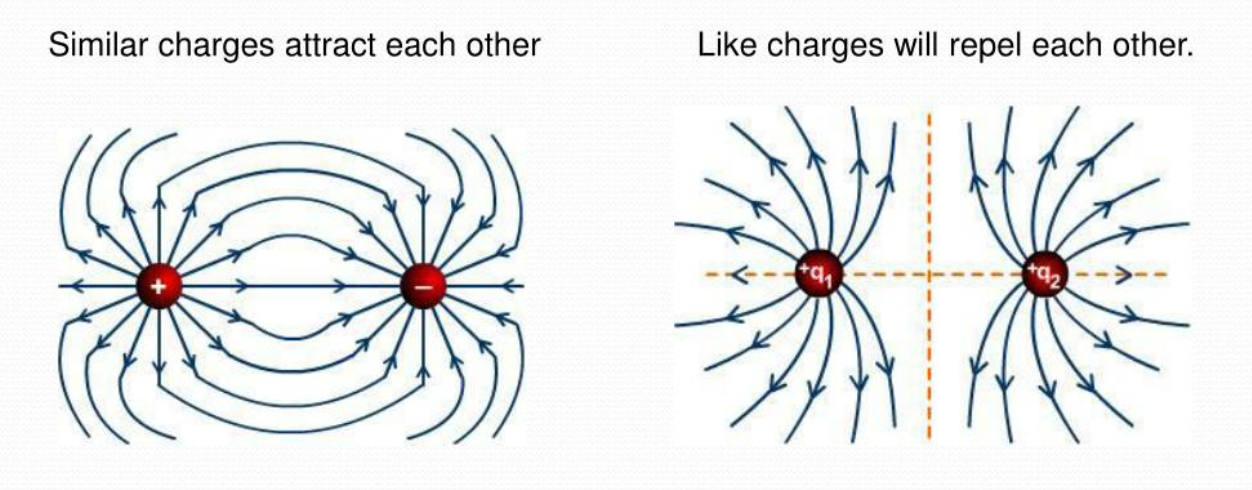
\includegraphics[width=0.9\linewidth]{phys12-electrostatics-field-lines-repulsion.png}
            \vspace{0.5cm}
            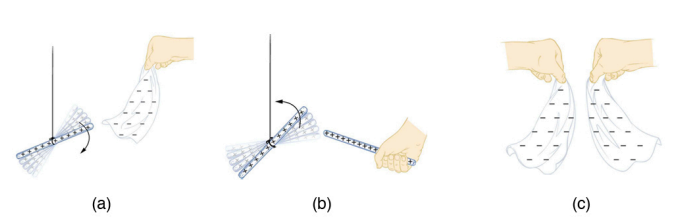
\includegraphics[width=0.9\linewidth]{phys12-electrostatics-charge-repulsion.png}
            \caption{Charge repulsion visualization}
        \end{figure}
\end{frame}

\begin{frame}
    \frametitle{Conservation of Charge}
    
    \begin{block}{Law of Conservation of Charge}
        \centering
        The net charge of an isolated system remains constant.\\
        \vspace{0.5em}
        \highlight{Charge cannot be created or destroyed.}
    \end{block}
    
    \begin{itemize}
        \item When an object becomes charged, it's due to a \highlight{transfer} of charge
        \item Common range for static electricity: nanocoulombs to microcoulombs
        \item Most charging results from \highlight{separation} of existing charges
        \item Example: Rubbing two neutral objects can transfer electrons
    \end{itemize}
    
    \begin{alertblock}{Important Equation}
        $Q_{system} = \sum q_i = \text{constant}$
    \end{alertblock}
\end{frame}

\begin{frame}{Charge Notation and Sources}
    \begin{columns}
        \column{0.6\textwidth}
        \begin{itemize}
            \item \textbf{Big Q} ($Q$):
                \begin{itemize}
                    \item Represents total or net charge
                    \item Measured in coulombs (C)
                    \item Used for describing overall charge of objects or systems
                    \item Source: Accumulation of multiple elementary charges
                \end{itemize}
            \item \textbf{Little q} ($q$):
                \begin{itemize}
                    \item Represents individual charge or point charge
                    \item Used in force calculations between charges
                    \item Source: Individual charged particles or concentrated charge
                \end{itemize}
            \item \textbf{Point charge} (a particle having a charge):
                \begin{itemize}
                    \item Idealized model where charge is concentrated at a single point
                    \item Creates an electric field in surrounding space
                    \item Exerts force on other charges according to Coulomb's law
                \end{itemize}
            \item \textbf{Test charge} ($q_0$):
                \begin{itemize}
                    \item Small positive charge used to measure electric fields
                    \item Assumed small enough not to disturb the existing field
                    \item Used to define electric field: $\vec{E} = \frac{\vec{F}}{q_0}$
                \end{itemize}
            \item \textbf{Elementary charge} ($e$):
                \begin{itemize}
                    \item Smallest discrete unit of charge
                    \item $e = 1.60 \times 10^{-19}$ C
                    \item Source: Electrons (negative) and protons (positive)
                \end{itemize}
        \end{itemize}
        
        \column{0.4\textwidth}
        \centering
        \begin{align}
            Q &= N \cdot e\\
            F &= k\frac{q_1 q_2}{r^2}\\
            \vec{E} &= \frac{1}{4\pi\varepsilon_0}\frac{q}{r^2}\hat{r}
        \end{align}
        \vspace{0.5cm}
    \end{columns}
\end{frame}

% Section: Conductors and Insulators
\section{Conductors and Insulators}

\begin{frame}
    \frametitle{Conductors vs. Insulators}
    
    \begin{columns}
        \column{0.5\textwidth}
        \textbf{Conductors:}
        \begin{itemize}
            \item Allow \highlight{free movement} of charge
            \item Electrons move easily through material
            \item Examples: metals (copper, aluminum)
            \item Excess charge distributes on surface
        \end{itemize}
        
        \column{0.5\textwidth}
        \textbf{Insulators:}
        \begin{itemize}
            \item \highlight{Restrict movement} of charge
            \item Electrons tightly bound to atoms
            \item Examples: rubber, plastic, glass
            \item Charge remains at placement location
        \end{itemize}
    \end{columns}
    
    \vspace{1em}
    \begin{block}{Semiconductors}
        Materials with properties between conductors and insulators
        (e.g., silicon, germanium)
    \end{block}
\end{frame}

\begin{frame}
    \frametitle{Polarization and Charging Methods}
    
    \textbf{Polarization:}
    \begin{itemize}
        \item Separation of positive and negative charges in a neutral object
        \item Induced by external electric field
        \item Creates local charge imbalances without overall charging
    \end{itemize}
    
    \vspace{0.5em}
    \textbf{Charging Methods:}
    \begin{itemize}
        \item \highlight{Charging by contact:} 
            \begin{itemize}
                \item Direct touch transfers charge
                \item Objects acquire same type of charge
            \end{itemize}
        \item \highlight{Charging by induction:}
            \begin{itemize}
                \item No direct contact required
                \item Requires grounding during process
                \item Objects acquire opposite type of charge
            \end{itemize}
    \end{itemize}
\end{frame}

% Section: Coulomb's Law
\section{Coulomb's Law}

\begin{frame}
    \frametitle{Coulomb's Law}
    
    \begin{block}{Coulomb's Law}
        The electrostatic force between two point charges is:
        \begin{equation}
            \vec{F} = k\frac{|q_1 q_2|}{r^2}\hat{r} \eqnlabel{18.1}
        \end{equation}
        where:
        \begin{itemize}
            \item $k = 8.99 \times 10^9$ N$\cdot$m$^2$/C$^2$ (Coulomb constant)
            \item $q_1, q_2$ are charges in coulombs
            \item $r$ is the distance between charges in meters
            \item $\hat{r}$ is the unit vector pointing from $q_1$ to $q_2$
        \end{itemize}
    \end{block}
    
    \begin{itemize}
        \item \highlight{Inverse-square} relationship with distance
        \item Similar to gravitational force, but \highlight{much stronger}
        \item Can be \highlight{attractive} (opposite charges) or \highlight{repulsive} (like charges)
    \end{itemize}
\end{frame}

\begin{frame}
    \frametitle{I Do: Coulomb's Law Example}
    
    \begin{exampleblock}{Example Problem}
        What is the repulsive force between two pith balls that are 8.00 cm apart and have equal charges of $-30.0$ nC?
    \end{exampleblock}
    \pause

    \begin{figure}
        \centering
        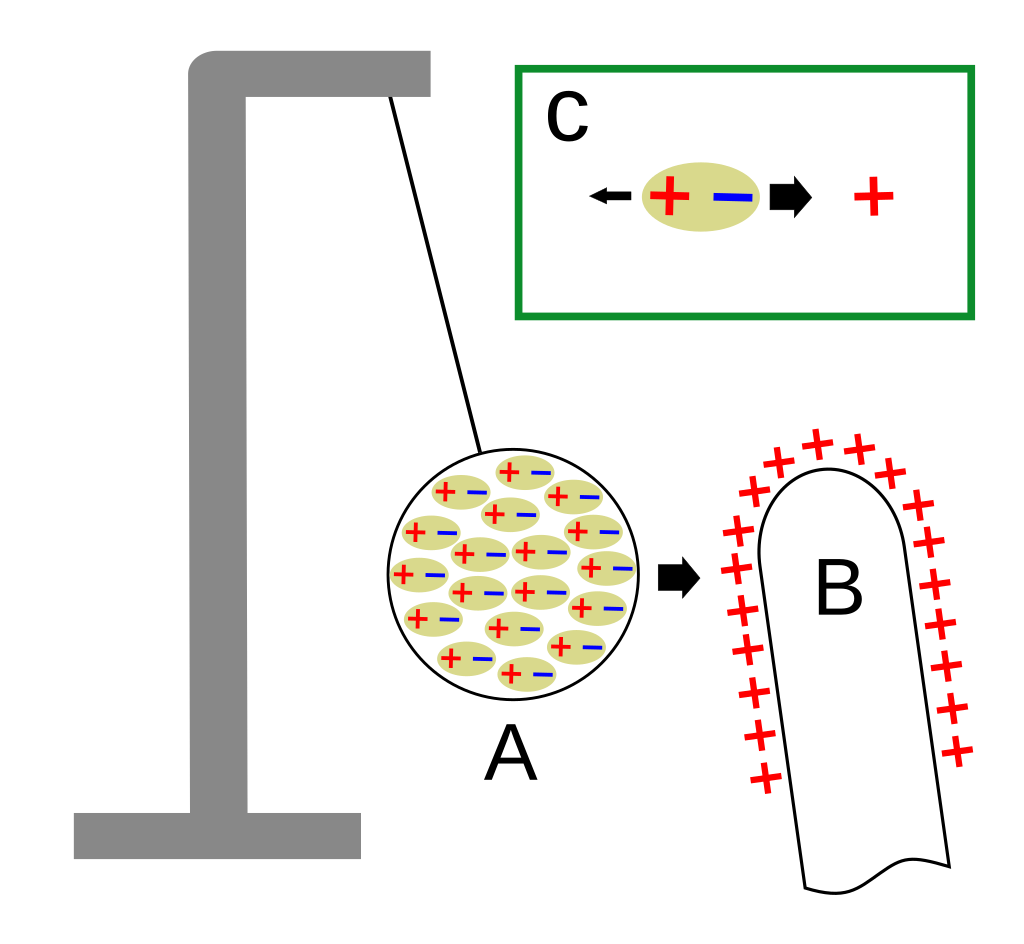
\includegraphics[width=0.4\linewidth]{phys12-electrostatics-pith-ball-electroscope.png}
    \end{figure}
\end{frame}
        

    \begin{frame}
    \frametitle{I Do: Coulomb's Law Example}
    
    \begin{exampleblock}{Example Problem}
        What is the repulsive force between two pith balls that are 8.00 cm apart and have equal charges of $-30.0$ nC?
    \end{exampleblock}
    \begin{block}{Solution}
        \begin{align}
            F &= k\frac{|q_1 q_2|}{r^2}\\
            &= (8.99 \times 10^9 \text{ N}\cdot\text{m}^2/\text{C}^2) \frac{(30.0 \times 10^{-9} \text{ C})^2}{(0.0800 \text{ m})^2}\\
            &= (8.99 \times 10^9) \frac{9.00 \times 10^{-16}}{6.40 \times 10^{-3}}\\
            &= 1.264 \times 10^{-3} \text{ N} \approx \highlight{1.27 \times 10^{-3} \text{ N}}
        \end{align}
    \end{block}
    
    \begin{itemize}
        \item The force is \highlight{repulsive} because the charges have the same sign
        \item This is a very small force, but measurable with sensitive equipment
    \end{itemize}
\end{frame}

% Section: Electric Field Concept
\section{Electric Field Concept}

\begin{frame}
    \frametitle{The Electric Field}
    
    \begin{block}{Electric Field Definition}
        The electric field $\vec{E}$ at a point in space is defined as the electric force $\vec{F}$ per unit charge that would act on a small positive test charge $q_0$ placed at that point:
        \begin{equation}
            \vec{E} = \frac{\vec{F}}{q_0} \eqnlabel{18.2}
        \end{equation}
    \end{block}
    
    \begin{itemize}
        \item Units: N/C (newtons per coulomb)
        \item A \highlight{vector} quantity with magnitude and direction
        \item Direction is the same as force on a \highlight{positive} test charge
        \item Exists at all points in space around charged objects
        \item Multiple electric fields \highlight{add vectorially}
    \end{itemize}
\end{frame}

\begin{frame}
    \frametitle{Electric Field of a Point Charge}
    
    \begin{block}{Electric Field of a Point Charge}
        The electric field created by a point charge $Q$ at a distance $r$ is:
        \begin{equation}
            \vec{E} = k\frac{|Q|}{r^2}\hat{r} \eqnlabel{18.3}
        \end{equation}
        where $\hat{r}$ points away from a positive charge or toward a negative charge.
    \end{block}
    
    \begin{itemize}
        \item Field strength \highlight{decreases} with the square of distance
        \item Field extends to infinity, but becomes weaker with distance
        \item The field of multiple charges is the \highlight{vector sum} of individual fields:
        \begin{equation}
            \vec{E}_{total} = \vec{E}_1 + \vec{E}_2 + \vec{E}_3 + \ldots \eqnlabel{18.4}
        \end{equation}
    \end{itemize}
\end{frame}

\begin{frame}
    \frametitle{We Do: Electric Field Example}
    
    \begin{exampleblock}{Example Problem}
        What is the magnitude and direction of an electric field that exerts a $2.00 \times 10^{-5}$ N upward force on a $-1.75$ μC charge?
    \end{exampleblock}
    \end{frame}

\begin{frame}
    \begin{block}{Let's Solve Together}
        Using the definition of electric field: $\vec{E} = \frac{\vec{F}}{q}$
        \begin{align}
            E &= \frac{F}{|q|}\\
            &= \frac{2.00 \times 10^{-5} \text{ N}}{1.75 \times 10^{-6} \text{ C}}\\
            &= 11.4 \text{ N/C}
        \end{align}
        
        For direction: Since the charge is \highlight{negative} and the force is \highlight{upward}, the electric field must be \highlight{downward}. 
        
        Remember: $\vec{F} = q\vec{E}$, and negative charges experience force in the direction \highlight{opposite} to the electric field.
    \end{block}
\end{frame}

% Section: Electric Field Lines
\section{Electric Field Lines}

\begin{frame}
    \frametitle{Electric Field Lines: Visualization}
    
    \begin{block}{Electric Field Lines}
        Visual representation of electric fields with the following properties:
    \end{block}
    
    \begin{itemize}
        \item Start on \highlight{positive} charges, end on \highlight{negative} charges
        \item Direction of field is \highlight{tangent} to the line at any point
        \item Density of lines proportional to field \highlight{strength}
        \item Number of lines from/to a charge proportional to charge \highlight{magnitude}
        \item Lines \highlight{never cross} (field has unique direction at any point)
    \end{itemize}
    
    \begin{figure}
        \centering
        \includegraphics[width=1\linewidth]{pointfields.png}
        \caption{Fig. 18.20}
    \end{figure}
\end{frame}

\begin{frame}
\begin{figure}
            \centering
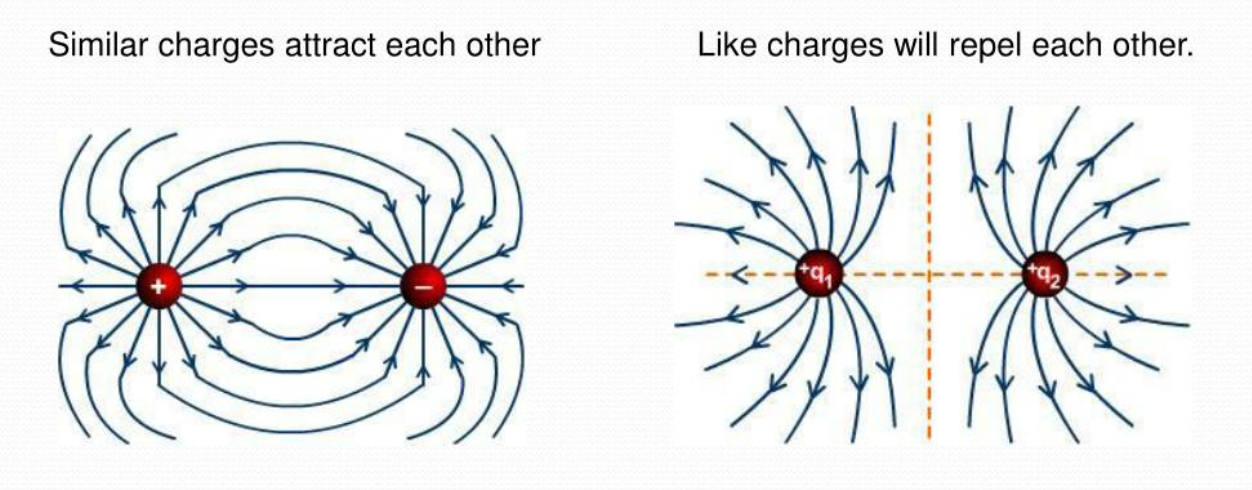
\includegraphics[width=1\linewidth]{phys12-electrostatics-field-lines-repulsion.png}
            \vspace{0.5cm}
          
        \end{figure}
\end{frame}

\begin{frame}
    \frametitle{Field Line Patterns}
    
    \begin{columns}[t]
        \column{0.5\textwidth}
        \textbf{Single Point Charge:}
        \begin{itemize}
            \item Positive charge: lines point \highlight{outward}
            \item Negative charge: lines point \highlight{inward}
            \item Radially symmetric pattern
        \end{itemize}
        
        \textbf{Two Like Charges:}
        \begin{itemize}
            \item Lines repel each other
            \item Field-free point between charges
        \end{itemize}
        
        \column{0.5\textwidth}
        \textbf{Two Unlike Charges:}
        \begin{itemize}
            \item Lines connect charges
            \item Concentrated between charges
            \item Form dipole field at distance
        \end{itemize}
        
        \textbf{Electric Dipole:}
        \begin{itemize}
            \item Equal + and - charges separated by small distance
            \item Important in molecular interactions
        \end{itemize}
    \end{columns}
\end{frame}

% Section: Conductors in Electrostatic Equilibrium
\section{Conductors in Electrostatic Equilibrium}

\begin{frame}
    \frametitle{Conductors in Electrostatic Equilibrium}
    
    \begin{block}{Key Properties}
        When a conductor reaches electrostatic equilibrium:
    \end{block}
    
    \begin{itemize}
        \item The electric field \highlight{inside} the conductor is \highlight{zero}
        \item Any excess charge resides \highlight{entirely on the surface}
        \item The electric field at the surface is \highlight{perpendicular} to the surface
        \item Charge concentrates at surfaces with greater \highlight{curvature}
        \item Charge density is highest at \highlight{sharp points} and edges
    \end{itemize}
    
    \begin{alertblock}{Implications}
        This explains why lightning rods have sharp points and why Faraday cages shield their interiors from external fields.
    \end{alertblock}
\end{frame}

\begin{frame}
    \frametitle{Lightning Rods and Faraday Cages}
    
    \textbf{Lightning Rods:}
    \begin{itemize}
        \item Metal rod with \highlight{sharp point}
        \item Facilitates charge \highlight{dissipation} into air
        \item Provides safe path to ground for lightning
    \end{itemize}
    
    \vspace{0.5em}
    \textbf{Faraday Cages:}
    \begin{itemize}
        \item Conducting enclosure shields interior from external field
        \item External charges induce surface charges that \highlight{cancel} internal field
        \item Applications: elevators, cars, microwave ovens, sensitive equipment
        \item \highlight{Protection} during lightning storms
    \end{itemize}
\end{frame}

% Section: Applications of Electrostatics
\section{Applications of Electrostatics}

\begin{frame}
    \frametitle{Practical Applications of Electrostatics}
    
    \begin{columns}[t]
        \column{0.5\textwidth}
        \textbf{Van de Graaff Generator:}
        \begin{itemize}
            \item Research and educational tool
            \item Generates high voltage, low current
            \item Can produce millions of volts
        \end{itemize}
        
        \textbf{Photocopiers \& Laser Printers:}
        \begin{itemize}
            \item Use charged drum
            \item Toner particles attracted to charged regions
            \item Heat fuses toner to paper
        \end{itemize}
        
        \column{0.5\textwidth}
        \textbf{Ink-Jet Printers:}
        \begin{itemize}
            \item Electrically charge ink droplets
            \item Deflect droplets to precise positions
        \end{itemize}
        
        \textbf{Electrostatic Air Filters:}
        \begin{itemize}
            \item Charge air particles
            \item Attract charged particles to plates
            \item Remove pollutants from air
        \end{itemize}
    \end{columns}
\end{frame}

\begin{frame}{}
    \begin{figure}
        \centering
        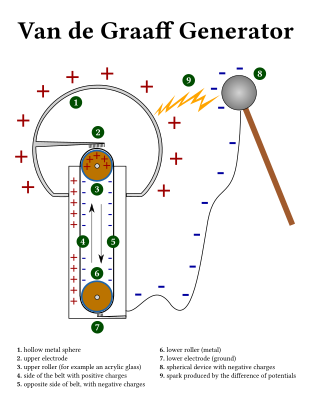
\includegraphics[width=0.6\linewidth]{phys12-electrostatics-van-de-graaff-generator.png}
    \end{figure}
\end{frame}

\begin{frame}
    \frametitle{You Do: Coulomb's Law Challenge}
    
    \begin{exampleblock}{Problem to Solve}
        Two point charges are brought closer together, increasing the force between them by a factor of 25. By what factor was their separation decreased?
    \end{exampleblock}
    
    \begin{itemize}
        \item Step 1: Recall Coulomb's law: $F = k\frac{|q_1 q_2|}{r^2}$
        \item Step 2: Set up ratio of forces: $\frac{F_2}{F_1} = 25$
        \item Step 3: Consider how distance affects the force
        \item Step 4: Solve for the ratio of distances
    \end{itemize}
    
    \begin{alertblock}{Work on this for 2 minutes}
        We'll discuss the solution afterward.
    \end{alertblock}
\end{frame}

\begin{frame}
    \frametitle{You Do: Solution}
    
    \begin{block}{Solution}
        From Coulomb's law:
        \begin{align}
            F_1 &= k\frac{|q_1 q_2|}{r_1^2} \quad \text{and} \quad F_2 = k\frac{|q_1 q_2|}{r_2^2}\\
            \frac{F_2}{F_1} &= \frac{r_1^2}{r_2^2} = 25\\
            \frac{r_1}{r_2} &= \sqrt{25} = 5
        \end{align}
    \end{block}
    
    \begin{itemize}
        \item Since $\frac{r_1}{r_2} = 5$, the separation was \highlight{decreased by a factor of 5}
        \item Remember: Force is inversely proportional to distance \highlight{squared}
        \item This is why the force increases so dramatically with small distance changes
    \end{itemize}
\end{frame}

% Summary slide
\begin{frame}
    \frametitle{Summary: Key Concepts}
    
    \begin{columns}[t]
        \column{0.5\textwidth}
        \textbf{Electric Charge:}
        \begin{itemize}
            \item Two types: positive and negative
            \item Like charges repel; unlike attract
            \item Conserved in isolated systems
        \end{itemize}
        
        \textbf{Coulomb's Law:}
        \begin{itemize}
            \item $F = k\frac{|q_1 q_2|}{r^2}$
            \item Inverse-square relationship
        \end{itemize}
        
        \column{0.5\textwidth}
        \textbf{Electric Field:}
        \begin{itemize}
            \item $E = \frac{F}{q}$ (force per unit charge)
            \item $E = k\frac{|Q|}{r^2}$ for point charge
            \item Field lines visualize direction and strength
        \end{itemize}
        
        \textbf{Conductors:}
        \begin{itemize}
            \item Excess charge on surface
            \item Zero field inside at equilibrium
            \item Charge concentrates at sharp points
        \end{itemize}
    \end{columns}
    
    
\end{frame}

% End slide
\begin{frame}
    \frametitle{Questions?}
    
    \begin{center}
        \Large{\highlight{Thank you for your attention!}}
        
        
    \end{center}
\end{frame}

\end{document}